\chapter{Gestión de Inventarios}
\section{Consideraciones generales}
\subsection{¿Qué son los stocks?}
Stock: Bienes y materiales que forman parte del activo de la empresa y que se acumulan para uso futuro con la finalidad de posibilitar la producción o satisfacer la demanda de los clientes.

Existencias: Mercancias almacenadas destinadas a venta. En contabilidad, la cuenta en la que se apuntan los movimientos relativos a los stocks. Por extensión se usa como sinónimo de stock.

Inventarios: Originalmente, lista de los bienes y materiales que componen el stock. Por extensión (y traducción directa de \textit{inventory}) se usa como sinónimo de stock.

\subsection{Tipos de inventarios}
Según el estado de transformación:
\begin{itemize}
    \item Suministros: materias primas, componentes, envases y embalajes, combustibles.
    \item Trabajo en curso (\textit{WIP: Work In Process}): han sufrido alguna transformación (o montaje) y están a la espera de completar el proceso productivo.
    \item Productos terminados: los que se venden a los clientes. También podríamos hablar de subproductos, que se obtienen durante la fabricación, pero no van incorporados al producto final.
\end{itemize}

Según su función:
\begin{itemize}
    \item Stock de desacoplamiento: inventario que separa procesos productivos y de cadenas de suministro.
    \item Stock de seguridad: inventario adicional para cubrir variabilidades en la demanda, el \textit{lead time}, y cantidad de lote recibida (\textit{buffer}).
    \item Stock cíclico: inventario derivado del tamaño del lote.
    \item Stock de anticipación (estacional): inventario acumulado para equilibrar la capacidad cuando hay demanda estacional.
    \item Stock en tránsito (\textit{pipeline}): inventario en proceso de transporte en la cadena de suministro.
    \item Stock especulativo: inventario acumulado ante expectativas de subidas de precio por especulación del mercado.
\end{itemize}

\subsection{¿Por qué no tener stocks?}
Necesitamos la cantidad adecuada de producto en el momento adecuado.

\begin{itemize}
    \item Costes que implican reducción de márgenes
    \item Dificultan las operaciones
    \begin{itemize}
        \item Entorpecen el flujo de materiales
        \item Malas prácticas
    \end{itemize}
    \item Ocultan problemas operativos
\end{itemize}

\section{Sistemas de gestión de inventarios}
El objetivo es mejorar el compromiso coste/nivel de servicio mediante reglas que regulen la forma de lanzar las órdenes de compra o producción de cada material.

Decisiones fundamentales:
\begin{itemize}
    \item Cuánto pedir: tamaño de lote
    \item Cuándo (cada cuánto) pedir: tiempo entre pedidos
\end{itemize}

¿Pedimos muchas veces poco o pocas veces mucho?

\subsection{Punto de pedido}
Cantidad de pedido fija: $Q$
Tiempo entre pedidos variable: $T_1, T_2, T_3,...$

\subsection{Revisión periódica}
Cantidad de pedido variable: $Q_1, Q_2, Q_3,...$
Tiempo entre pedidos fijo: $T$

\begin{figure*}
    \centering
    \begin{subfigure}[c]{0.45 \textwidth}
        \centering
        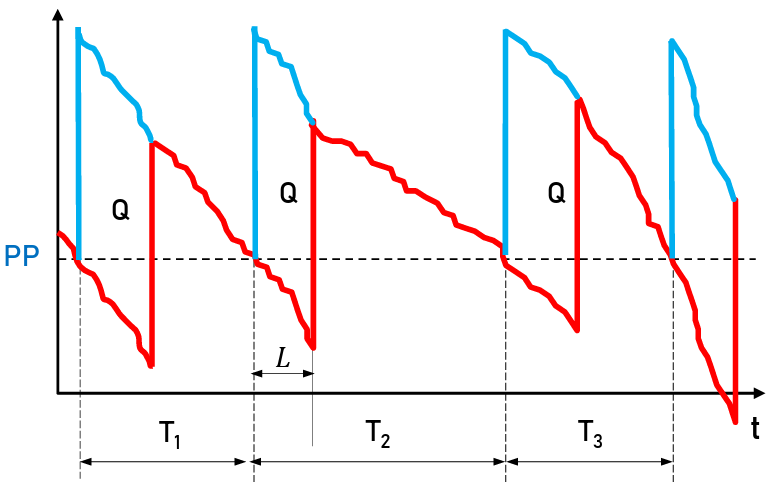
\includegraphics[width = \textwidth]{Imagenes/Tema 3. Punto de pedido.png}
        \caption{Punto de pedido}
    \end{subfigure}
    \hfill
    \begin{subfigure}[c]{0.45 \textwidth}
        \centering
        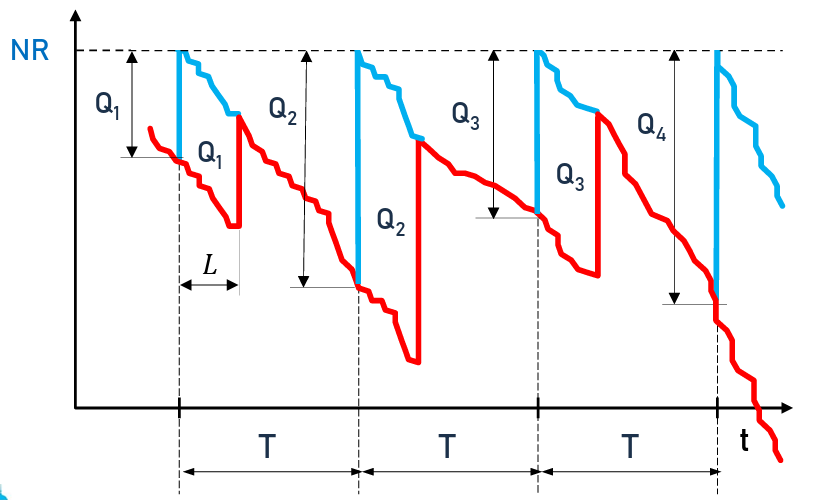
\includegraphics[width = \textwidth]{Imagenes/Tema 3. Revision periodica.png}
        \caption{Revisión periódica}
    \end{subfigure}
    \caption{Políticas básicas}
\end{figure*}

Aspectos relevantes a tener en cuenta:
\begin{itemize}
    \item Tipo de demanda
    \begin{itemize}
        \item Independiente vs. dependiente
        \item Determinista vs. no determinista
    \end{itemize}
    \item Políticas de gestión
    \begin{itemize}
        \item Cuánto pedir / cuándo pedir
        \item Revisión continua / periódica
    \end{itemize}
    \item \textit{Lead time} (plazo de entrega)
    \item Horizonte temporal
    \item Restricciones (capacidad, tamaño de lote)
    \item Costes relevantes
\end{itemize}

\section{Costes en gestión de inventarios}
\subsection{Aprovisionamiento}
Coste de emisión ($S \times nº\ de\ pedidos$)


\subsection{Tenencia}

\subsection{Roturas de inventario}

\section{Modelos deterministas}
\subsection{Modelo EOQ}

\subsection{Descuentos por cantidad}

\section{Modelos probabilistas}
\subsection{Stock de seguridad}

\subsection{Nivel de servicio}

\section{Control de inventarios}